\section{Análise GRASP}

O Zend Framework é um grande exemplo de utilização de padrões de
projeto.

\subsection{Caso de Uso: Novo Documento}

Para o caso de uso Novo Documento precisamos de um Controlador, um
Criador e um Especialista. Vejamos a figura
\ref{dia-seq-novo-documento}.

\begin{figure}[h]
    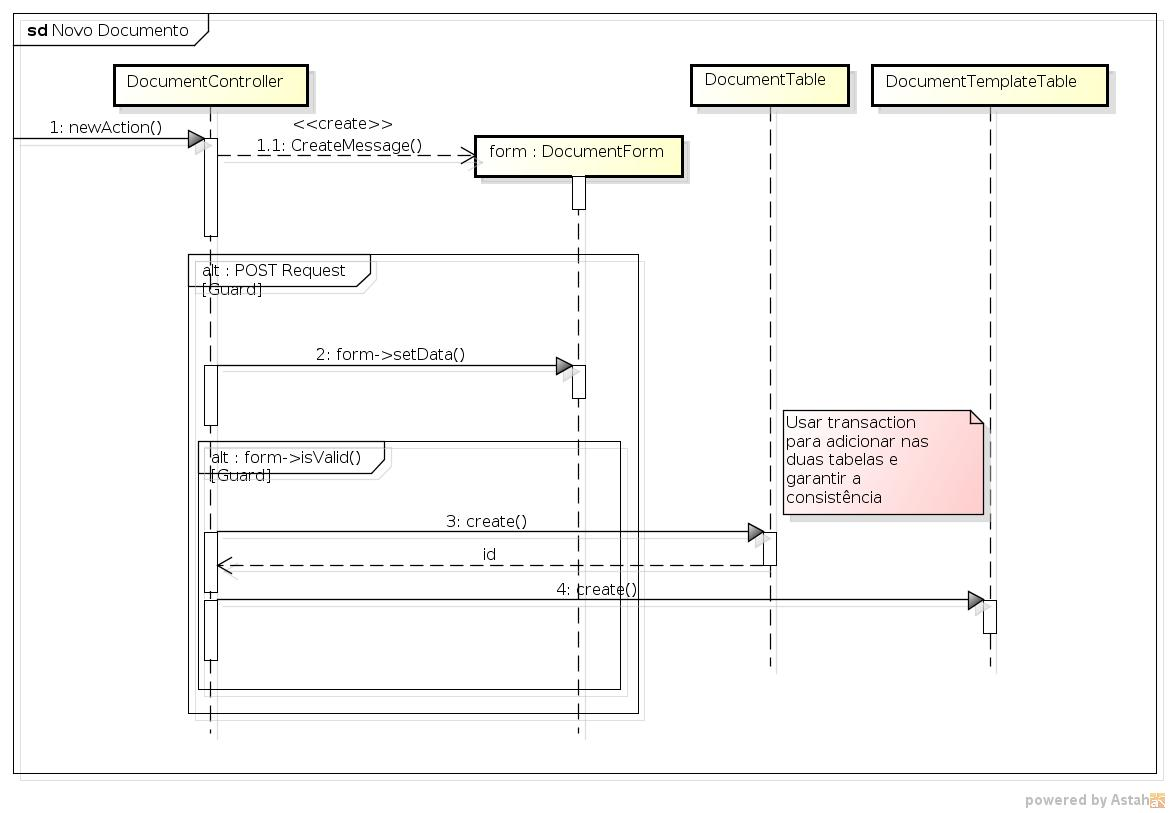
\includegraphics[scale=0.4]{img/DiagramaSequenciaNovoDocumento.jpg}
    \caption{Dia. Seq. Novo Documento}
    \label{dia-seq-novo-documento}
\end{figure}

Nela podemos ver de cara o padrão Controlador na classe
\textbf{DocumentController}. Ela é uma classe que extende de
\textbf{AbstractActionController}, que faz parte do Zend Framework. É a
classe responsável por capturar a interação do usuário e delegar os
eventos para uma determinada \textbf{Action} (ação). Veja que a chamada
que origina tudo é \textbf{newAction}. No Zend sempre que você colocar
\textbf{Action} no final do método, quer dizer que esse método é uma
ação que o controlador deve receber e tratar.

Em seguida o controlador cria o Formulário \textbf{NewDocument}. É
função do controlador criar o formulário sempre que a ação
\textbf{newAction} for requisitada. Aqui podemos ver o padrão criador
sendo executado pelo controlador.

Existe ainda um especialista que não está presente no diagrama mas é de
extrema importância, o ServiceManager. Segundo a
\href{http://framework.zend.com/manual/2.0/en/modules/zend.service-manager.quick-start.html}{documentação}
ele é responsável por prover:

\begin{itemize}
\item
  Fábricas abastratas
\item
  \emph{Aliases}
\item
  Fábricas
\item
  \emph{Invokables}
\item
  Serviços
\item
  Serviços Compartilhados
\end{itemize}
No controlador \textbf{DocumentController} ele tem como objetivo obter
uma instância de \textbf{TemplateTable} e
\textbf{DocumentTemplateTable}, dois \textbf{Models} do sistema; obter
um objeto de \textbf{Sessão}, contendo os dados do usuário logado; e
obter o \textbf{Adapter} do banco de dados, responsável pela conexão,
para que possamos criar uma transação na hora de criar o documento,
devido a necessidade de inserir dados em duas tabelas diferentes. Ex.:

\begin{verbatim}
/* ... */
$sm = $this->getServiceLocator();
$modelTemplates = $sm->get('Application\Model\TemplateTable');

if ($request->isPost()) {
    $session = $sm->get('Session');
    /* ... */
}
\end{verbatim}

